% ReRide README abstract, adapted from the recovered exploration.
% 246.175 x 123.0875 mm page (2:1); artwork is placed without stretching.
% Black linework only. Artwork provides unshaded orthographic component views.
% Final PDF export additionally uses Ghostscript DeviceGray conversion.
% Native sensor coordinates prevent left/right placement and count errors.
\documentclass[tikz,border=0pt]{standalone}
\usepackage[T1]{fontenc}
\usepackage{helvet}
\renewcommand\familydefault{\sfdefault}
\usepackage{graphicx}
\usetikzlibrary{arrows.meta}
\tikzset{every node/.style={font=\fontsize{9}{10.5}\selectfont,
  text=black,align=center,inner sep=0pt},
  flow/.style={draw=black,line width=.6pt,
    -{Stealth[length=1.2mm,width=.95mm]},rounded corners=1.5mm},
  detail/.style={draw=black,line width=.5pt,fill=white}}
\newcommand{\fiducial}[2]{
 \begin{scope}[shift={(#1,#2)}]
  \fill[white] (-15,-15) rectangle (15,15);
  \fill[black] (-13,-13) rectangle (13,13);
  \fill[white] (-9,-9) rectangle (9,9);
  \fill[black] (-9,-9) rectangle (-3,-3);
  \fill[black] (-3,-3) rectangle (3,3);
  \fill[black] (3,-9) rectangle (9,3);
  \fill[black] (-9,3) rectangle (3,9);
 \end{scope}}
\begin{document}
\begin{tikzpicture}[x=.1075mm,y=-.1075mm]
\path[use as bounding box] (-145,-12.5) rectangle (2145,1132.5);
\node[anchor=north west] at (0,0)
 {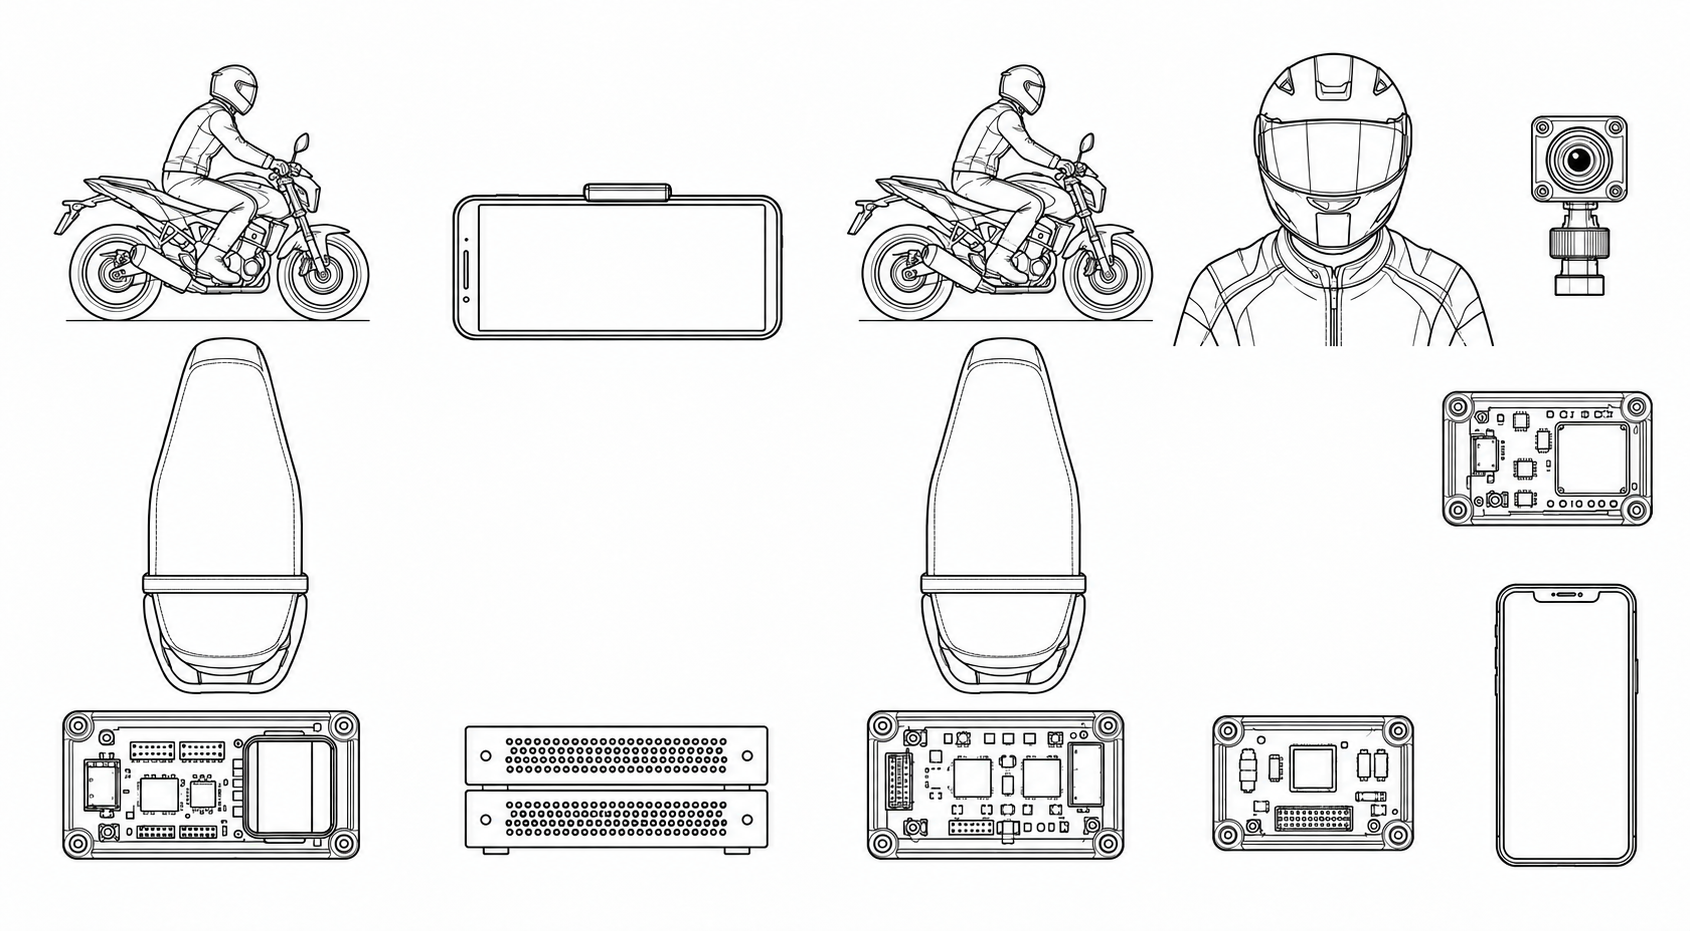
\includegraphics[width=215mm]{artwork-original.png}};
\draw[black,line width=.3pt] (1005,34)--(1005,1110);

% Both seats face front-up. The first pair shares EXACTLY the same y value.
\foreach \x in {230,300}{
 \draw[detail] (\x-16,609) rectangle (\x+16,641);
 \draw[black,line width=.3pt] (\x-12,613) rectangle (\x+12,637);
}
% Six sites: three longitudinal rows, two left/right positions per row.
\foreach \y in {521,592,651}{
 \foreach \x in {1154,1224}{\draw[detail] (\x,\y) circle (10);}}
% Front-view marker locations: helmet, chin, left shoulder, right shoulder.
\fiducial{1580}{105}\fiducial{1580}{273}
\fiducial{1450}{337}\fiducial{1720}{337}

% Monochrome schematic screen glyphs, not measurements or a reconstructed UI.
\draw[black,line width=.4pt] (790,250)--(790,385);
\draw[black,line width=.45pt] (575,327)--(602,327)--(602,291)
 --(634,291)--(634,347)--(661,347)--(661,312)--(695,312)
 --(695,330)--(730,330)--(730,280)--(768,280);
\draw[black,line width=.5pt] (846,316) circle (39);
\draw[black,line width=.4pt] (846,277)--(846,316)--(882,332);
\draw[black,line width=.3pt,densely dotted]
 (1855,733)--(1855,985) (1799,855)--(1923,855);
\draw[black,line width=.6pt] (1855,782)
 .. controls (1884,779) and (1872,821) .. (1892,836)
 .. controls (1943,885) and (1895,914) .. (1863,928)
 .. controls (1798,964) and (1791,904) .. (1810,874)
 .. controls (1835,838) and (1789,802) .. (1855,782);

\node[anchor=west] at (50,40) {INTERACT 2017};
\node[anchor=west] at (400,625) {2 pressure sensors};
\node[anchor=south] at (740,197) {Live history\\and ride summary};
\node[anchor=north] at (265,1055) {Genuino};
\node at (735,1114) {Bluetooth};
\node[anchor=north] at (790,1028) {Remote storage};
\draw[flow] (265,823)--(265,840);
\draw[flow] (426,930)--(490,930)--(490,1082)--(970,1082)
 --(970,300)--(925,300);
\draw[flow] (830,404)--(830,810)--(790,810)--(790,858);

\node[anchor=west] at (1050,40) {TEI 2019 (BANk)};
\node[anchor=west] at (1320,595) {6 pressure sites};
\node[anchor=south] at (1580,45) {4 fiducial markers};
\node[anchor=south] at (1880,115) {Upper-body\\camera};
\node[anchor=east] at (1678,550) {Camera sensing\\(Pi)};
\node[anchor=north] at (1185,1055) {Seat sensing\\(2 ADCs + Pi)};
\node[anchor=north] at (1555,1055) {Central processing};
\node[anchor=north] at (1855,1055) {Glanceable\\posture};
\node[anchor=south] at (1855,650) {WebSockets};
\draw[flow] (1880,350)--(1880,465);
\draw[flow] (1189,823)--(1189,841);
\draw[flow] (1331,925)--(1438,925);
\draw[flow] (1952,550)--(1980,550)--(1980,668)--(1700,668)
 --(1700,810)--(1560,810)--(1560,847);
\draw[flow] (1677,925)--(1770,925);
\end{tikzpicture}
\end{document}
